
\chapter{Artificial Neural Network}
An artificial \gls{neuralnet} is constructed as shown in figure
\ref{fig:ann_ex}. Where one has the input layer on the bottom which takes a set
of input values an propagates them to the next layer.  This next layer is the
first of one or more layers that propagates the input values through many
weighted \gls{synapse}s which have been through the \gls{perceptron}s activaiton
function.  After passing through the entire hidden layer, the values comes tho
the output layer which will calculate the output value.

After this the software calculates the errors for each of the outputs and
decides whether it has converged.  All output nodes that has converged are
marked and when all nodes has converged, the entire network has converged and
should provide the desired output.

\section{Perceptrons (Nodes)}
The \gls{perceptron} is the junction points in the network where the outputs of
the previous layer is pushed into the new layer. The \gls{perceptron} receives the
weighted outputs of the previous layer and stores the sum of all its inputs.

The input is then pushed through the activation function of the \gls{perceptron},
which generates the \gls{perceptron}s output value. This output value is the value
which is passed on to the next layer through the \gls{synapse}s. As it passes throught
he \gls{synapse}s it's weighted and the resulting value is pushed to the linked 
\gls{perceptron}.


\begin{figure}[b]
\centering
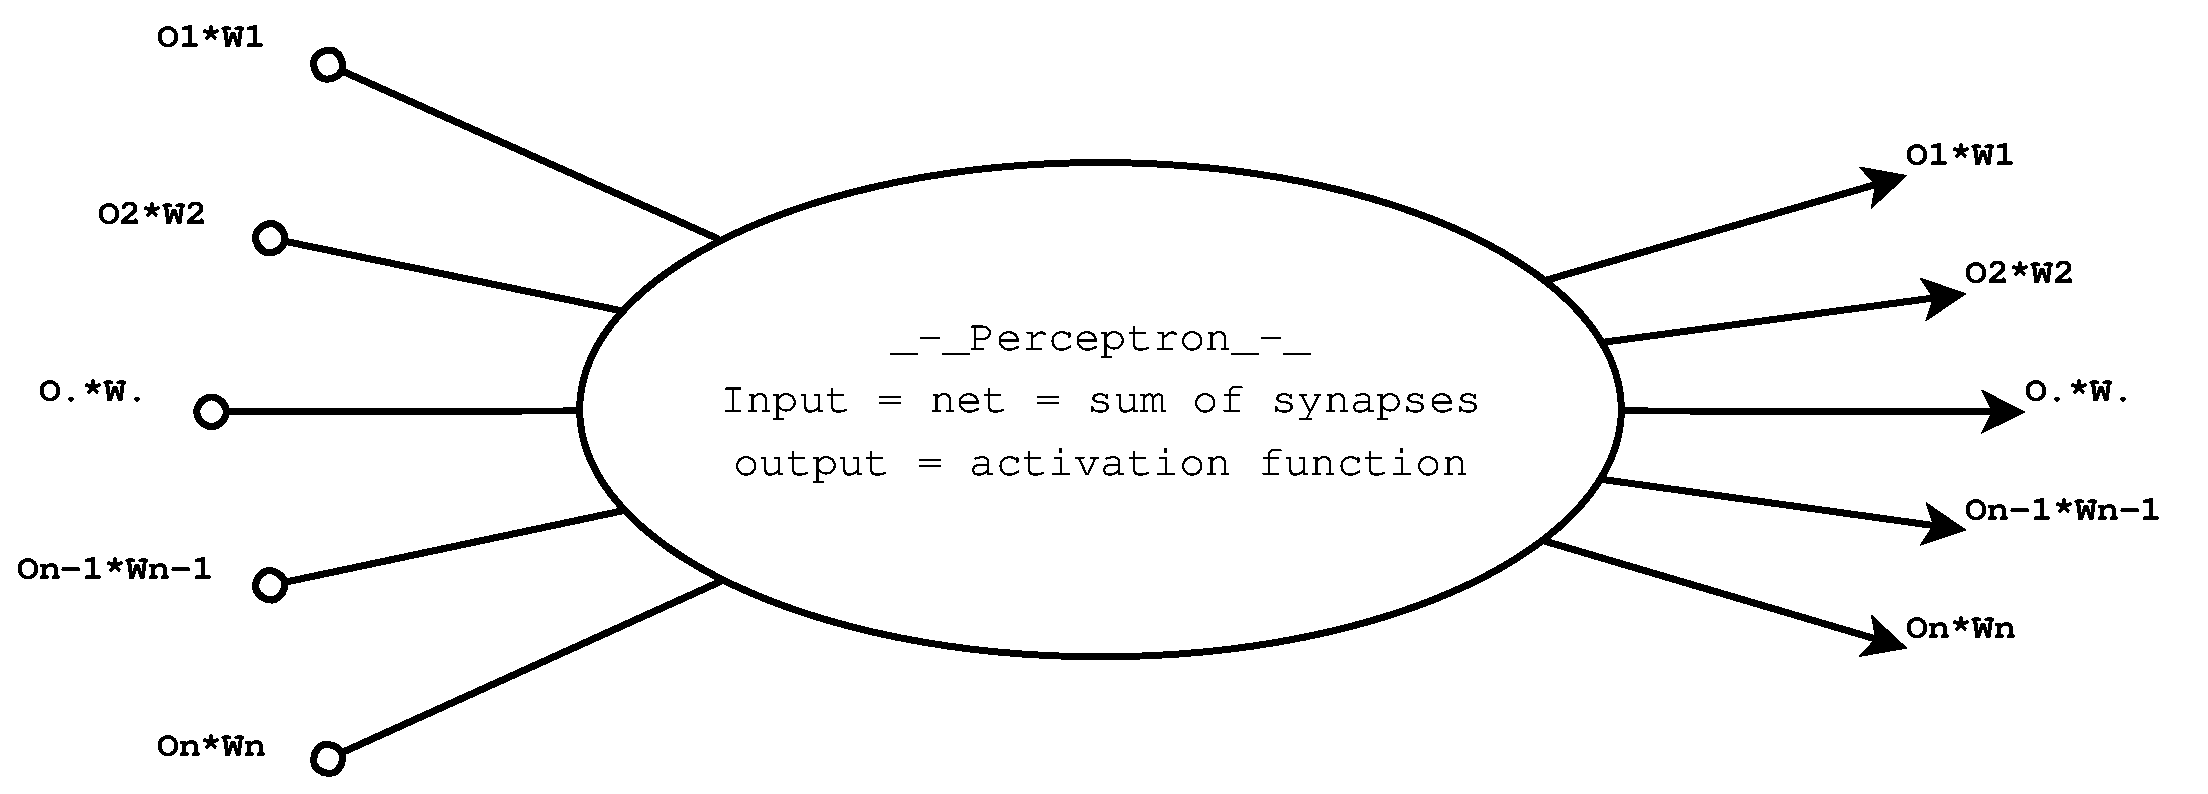
\includegraphics[width={0.9\textwidth}]{pictures/perceptron}
\caption{Illustration of a \gls{perceptron} with n inputs and n outputs}
\label{fig:perceptron}
\end{figure}

\subsection{Activation function}
\gls{actfunc} is a mathematical operation that takes the net input and
calculates an output value. The most used functions is the hyperbolic tan
function and the \gls{sigmoid} function. The function which we use are the
sigmoid function which generates a value between -1 and +1 from the net input
value.  It uses the function, $1\div(1+e^{-net})$ to generate the output value.


\subsection{Software representation}
We have created a representation of a \gls{perceptron} with the class ''Node'',
which is depictedn in figure \ref{fig:uml_weight}, using UML to describe it. It
has a set of variables which holds the information and state of the node.

\begin{longtable}{ p{0.2\textwidth}  p{0.7\textwidth} }
\textbf{id} 		& 	This is the integer id of the perceptron(node), and is only unique
	within the layer it is in. It is mostly used for identification, but also for
	making it easy to insert new values from the data structure, since it can
	retrieve its id from the value array.\\
\textbf{input}	& 	This is a float value which represents the input value from
	either from the data set or the weighted outputs from the previous layer.\\
\textbf{output}	& 	This holds the output value created by the activation
	function of the node. For most layers that is the sigmoid function, but also a
	custom function to decide the output from the input layer.\\
\textbf{error}	& 	This holds the error returned from the error calculation
	function, as a part of the backpropagation algorithm.  This is then used by
	the lower layer to adjust its weights linking to the layer.\\
\textbf{*weight}& 	This is a pointer to the first element of a list containing
	the set of weights connecting it to the next layer.\\
\textbf{*next}	& 	This is a pointer to the next instance of a object in the
	list of Nodes(layer), the last instance in the list will point to ''NULL''.\\
\textbf{convergence} &	This is a boolean value stating whether or not the Node
	has reached convergence as desired by the output.\\
\end{longtable}



\section{Synapses (Links)}
A \gls{synapse} is the directed link between to \gls{perceptron}s. It's purpose
is to weight the signal passing through it to give a better result to the
output. As the neural network training progresses this weight changes to provide
the best end output for the overall network.  The change is made using the
backpropagation algorithm, see chapter \ref{chp:backprop}.


\subsection{Software representation}
We have created a representation of the synapses with the class ''Weight'' which
is depicted in figure \ref{fig:uml_node}, using UML to describe it.  It has a
set of variables to hold the information and make it possible to use te
backpropagation algorithm. It also have a set of methods to help with retrieving
the information in order to facilitate the algorithm.

The ''Weights'' is a member of the perceptron and forms a list of all
connections the perceptron has a connection to.

\begin{longtable}{ p{0.1\textwidth}  p{0.8\textwidth} }
\textbf{id} &			The id is an auto incremented counter that identifies which
	weight we are currently accessing in the list. Mostly used for identifying
	the weight/synapse during information display. \\
\textbf{to} &			This variable is a pointer, which points to the perceptron(node)
	that the synapse(weight) connects to. This is used to grab a hold of the
	linked node when pushing the input value through the network and so on. And
	must be here since it is a \gls{FF} network. \\
\textbf{weight} &	This is a float value that holds the current weight value of the
	synapse. This is the weight that is used when propagating the input value
	through the network.\\
\textbf{change} &	This is a float value that holds the value of the previous
	weight change. This value is decided when calculating the weight change
	during backpropagation. The change value is then multiplied by the momentum, a
	small decimal value.\\
\textbf{next} &		This is a pointer to the next Weight in the list. The last
	element in the list will point to ''NULL''.\\
\end{longtable}


\section{Construction}
After a couple of tries we decided to create a fully connected ANN(Artificial
Neural Network). This means that every perceptroon on the previous layer has a
synapse to each perceptron on the next layer. As depicted in figure
\ref{fig:ann_ex}.

For our network we have created a general implementation which makes it possible
to create a input layer, arbitrary amount of hidden layers and a output layer.
The input and output layer can have arbitrary amounts of nodes, but the hidden
layers must all have the same amount of nodes.

For our network we have created a network with 100 input perceptrons and 26
output perceptrons. The hidden layer is then chosen to have an arbitrary amount
of nodes and layers so we could test different implementations.

\begin{figure}[h]
\centering
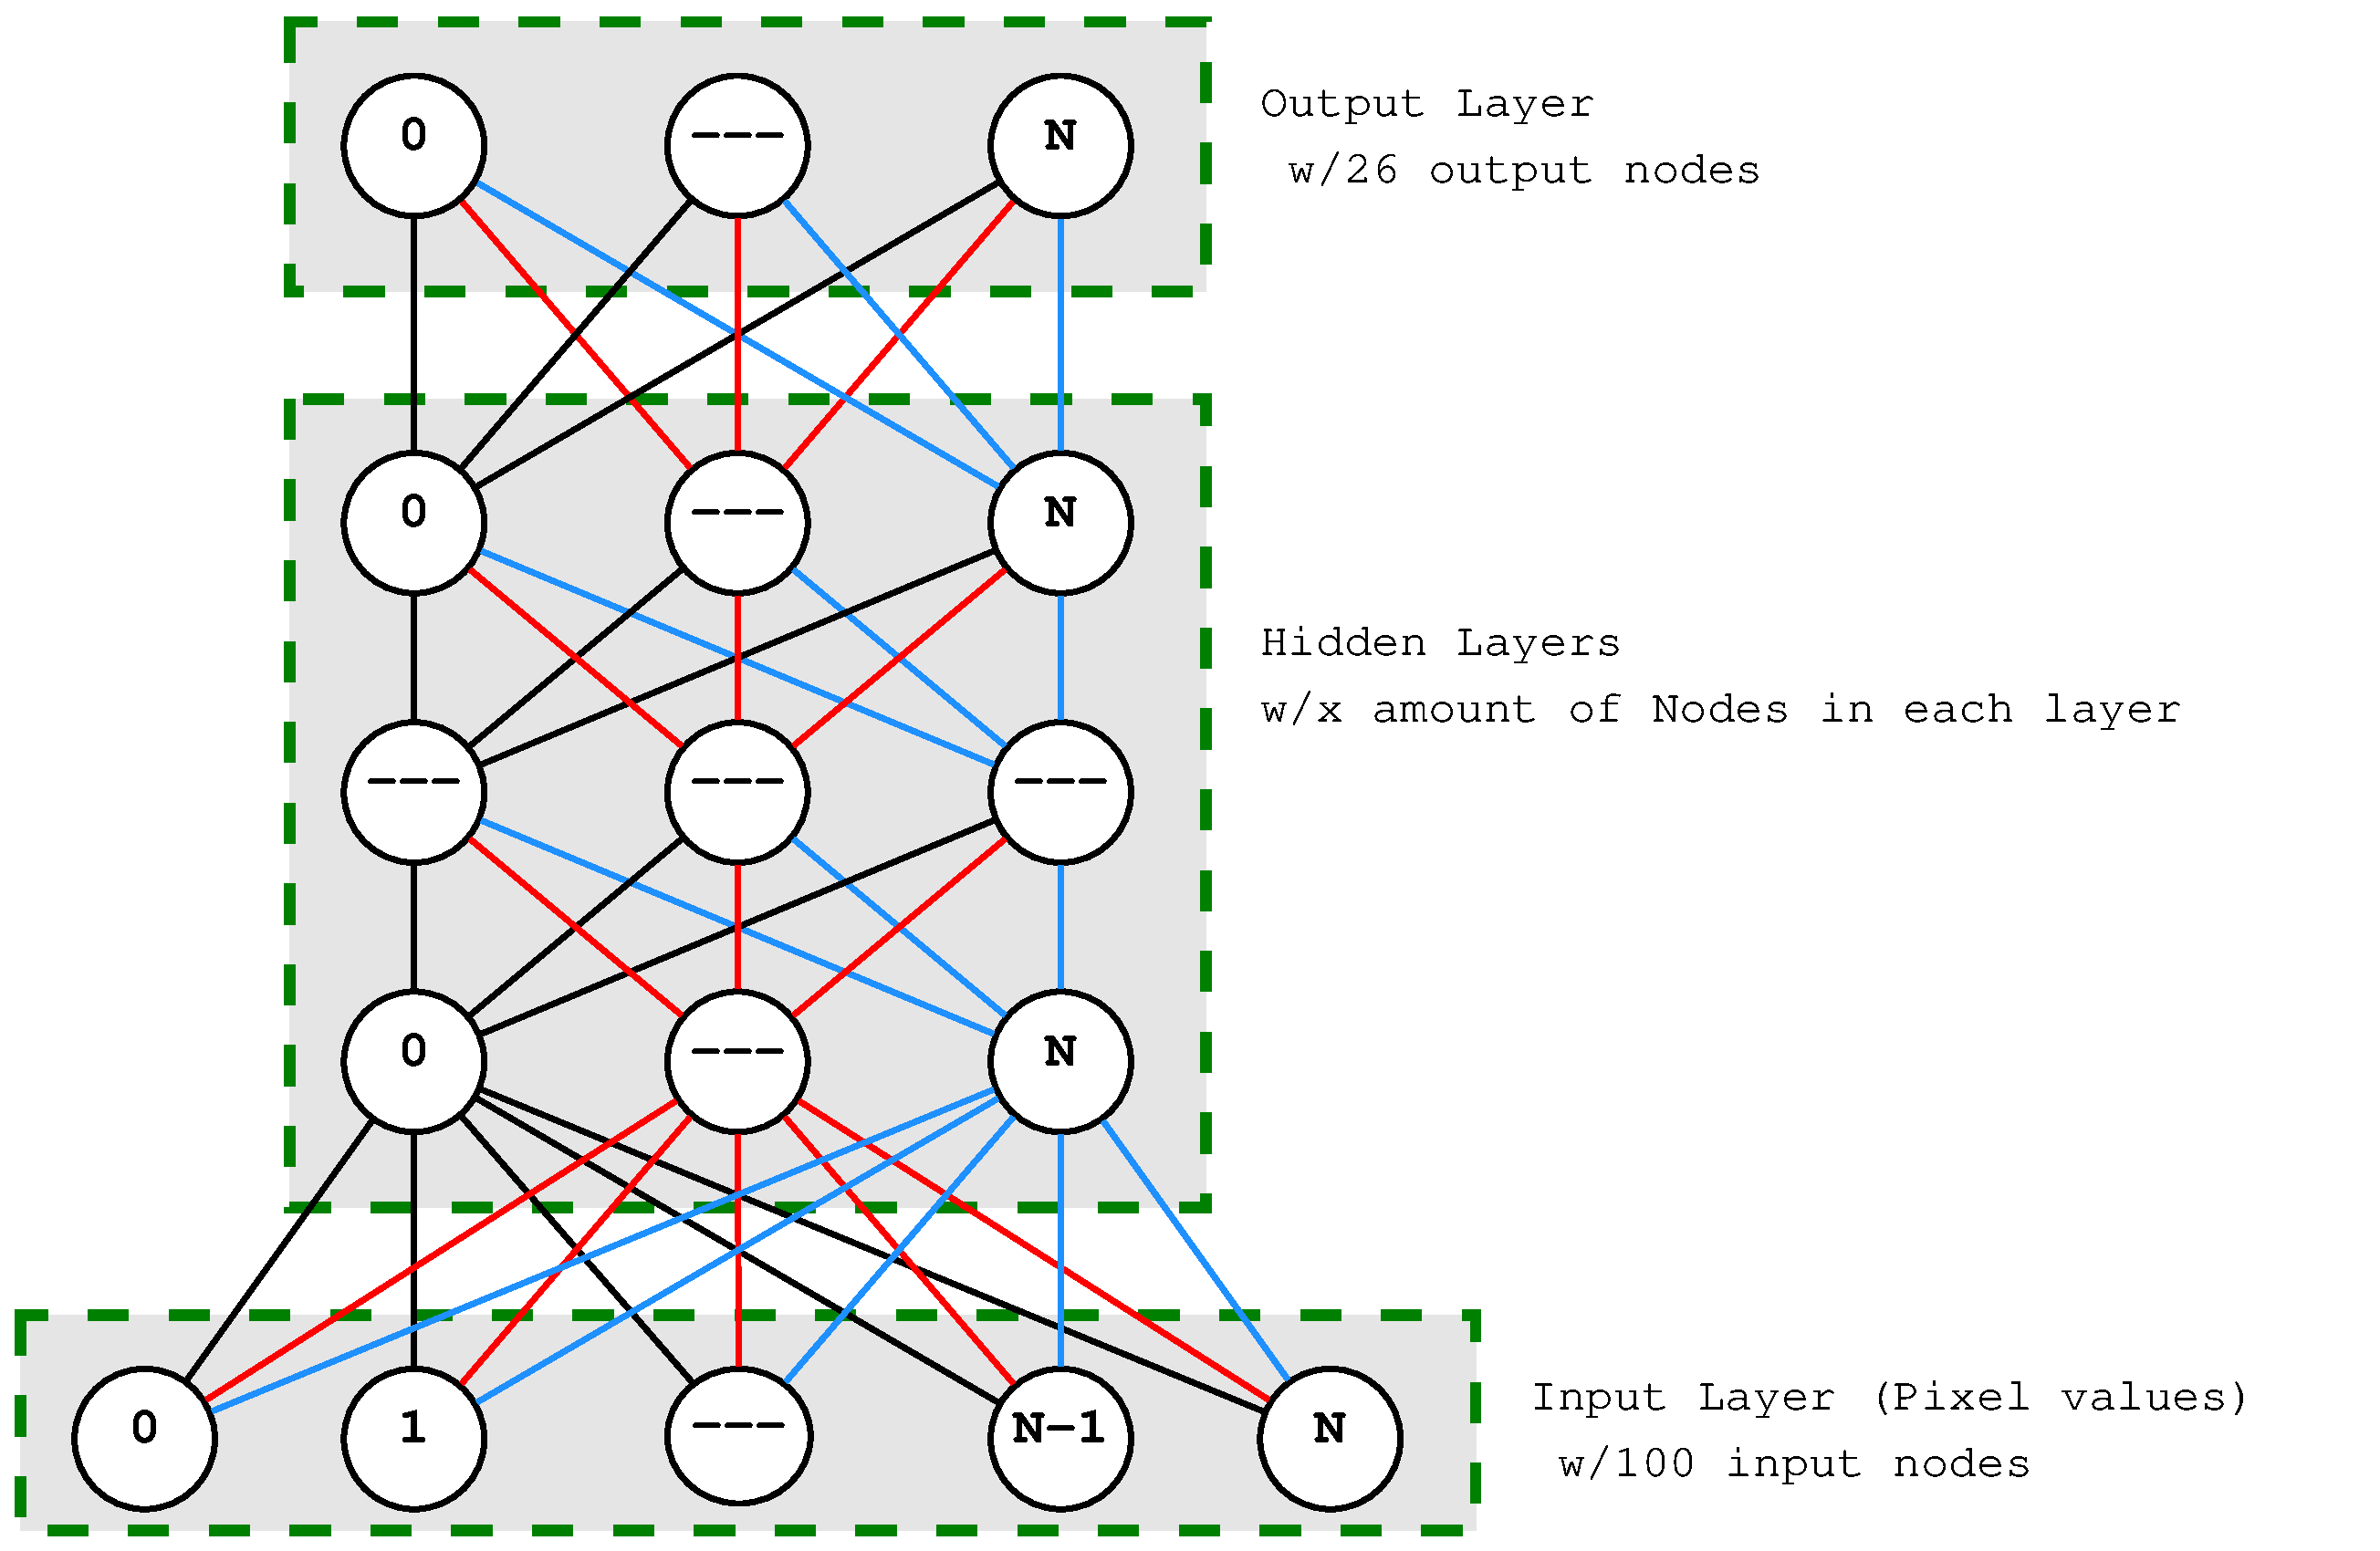
\includegraphics[width={0.9\textwidth}]{pictures/network}
\caption{Illustration of a fully connected, neural network}
\label{fig:ann_ex}
\end{figure}

The network construction starts by creating the input layer. It creates a list of
Node objects that starts at the global ''input'' pointer, which makes it easy to
grab a hold of and use later. Then it does the same for each of the hidden
layers and output layer.

Once this is finished we have a set of lists made up by Node objects, depicting
perceptrons, but none of them are linked to eachother. This is the next step.

We start with the input list, and grab the global pointer which points to the
first object of the list.  Then we call a the Nodes local method, ''setWeight''.
It takes one parameter, a pointer to a Weight object.  This pointer should then
point to a list of Weight objects that has links to the next layer of nodes.

This is done by calling it in the following manner:
\begin{verbatim}
input->setWeight( genWeights( NUM\_IN\_HIDDEN, hidden[0] ));
\end{verbatim}

Here we call the genWeights funciton which takes a int and a list of
\gls{perceptron}s
as input. It then generates a list of Weight-objects with random weights that
links to the provided layer of nodes.

This way we create for each Node full connection to the next layer.


\subsection{Input Layer}
We chose to use a 100 input \gls{perceptron}s because it provided a reasonable amount
of accuracy in the images data to recreate the picture without loosing the
information.

To set the input values we have a function that we call on the ''input'' layer.
''setInputs'' which then will call getValue on the global inData object, using
its id as paramater. This enables it to consequently and easily retrieve the
same index each time.

\subsection{Hidden layers}
There are no special functionality surrounding the hidden layer, except when we
are updating weights, which is mostly done through the hidden layers.

\subsection{Output Layer}
The output layer consists of 26 perceptons because it makes it easy to see what
charachters the input data is classified as.  Since we want a value between 0
and for each output perceptron we can multiply by 100 and get the percentage of
classification for the data being a specific character.

The output the tests yields is in the form below. This example says that it has
classified the input data as 20\% similar to a 'U', 58\% similar to a 'G', 40\%
similar to 'D', 90\% similar to 'C' and 20\% similar to a 'B'.
Because of this on can confident that it is a 'C'.
\begin{longtable}{
	p{0.05\textwidth} p{0.02\textwidth} p{0.02\textwidth} p{0.02\textwidth} 
	p{0.02\textwidth} p{0.02\textwidth} p{0.02\textwidth} p{0.02\textwidth} 
	p{0.02\textwidth} p{0.03\textwidth} p{0.02\textwidth} p{0.02\textwidth} 
	p{0.02\textwidth} p{0.02\textwidth} p{0.02\textwidth} p{0.02\textwidth} 
	p{0.02\textwidth}
}
CHAR&id&Z&Y&X&W&V&U&T&....&H&G&F&D&C&B&A\\\hline
C&4&0\%&0\%&0\%&0\%&0\%&20\%&0\%&....&0\%&58\%&0\%&40\%&90\%&20\%&0\%\\

\end{longtable}


